% Options for packages loaded elsewhere
\PassOptionsToPackage{unicode}{hyperref}
\PassOptionsToPackage{hyphens}{url}
\PassOptionsToPackage{dvipsnames,svgnames*,x11names*,table}{xcolor}
%
\documentclass[
  ignorenonframetext,
]{beamer}
\usepackage{pgfpages}
\setbeamertemplate{caption}[numbered]
\setbeamertemplate{caption label separator}{: }
\setbeamercolor{caption name}{fg=normal text.fg}
\setbeamertemplate{bibliography item}{\insertbiblabel}
\beamertemplatenavigationsymbolsempty
% Prevent slide breaks in the middle of a paragraph
\widowpenalties 1 10000
\raggedbottom
\setbeamertemplate{part page}{
  \centering
  \begin{beamercolorbox}[sep=16pt,center]{part title}
    \usebeamerfont{part title}\insertpart\par
  \end{beamercolorbox}
}
\setbeamertemplate{section page}{
  \centering
  \begin{beamercolorbox}[sep=12pt,center]{part title}
    \usebeamerfont{section title}\insertsection\par
  \end{beamercolorbox}
}
\setbeamertemplate{subsection page}{
  \centering
  \begin{beamercolorbox}[sep=8pt,center]{part title}
    \usebeamerfont{subsection title}\insertsubsection\par
  \end{beamercolorbox}
}
\AtBeginPart{
  \frame{\partpage}
}
\AtBeginSection{
  \ifbibliography
  \else
    \frame{\sectionpage}
  \fi
}
\AtBeginSubsection{
  \frame{\subsectionpage}
}
\usepackage{lmodern}
\usepackage{amssymb,amsmath}
\usepackage{ifxetex,ifluatex}
\ifnum 0\ifxetex 1\fi\ifluatex 1\fi=0 % if pdftex
  \usepackage[T1]{fontenc}
  \usepackage[utf8]{inputenc}
  \usepackage{textcomp} % provide euro and other symbols
\else % if luatex or xetex
  \usepackage{unicode-math}
  \setmainfont[]{Noto Sans CJK JP}
  \setsansfont[]{Noto Serif CJK JP}
  \setmonofont[]{Ricty}

% japanese font setting
% if the preset is specified
\ifxetex
  \usepackage[AutoFallBack=true]{zxjatype}
  \usepackage[noto,]{zxjafont}
  \usepackage{xeCJKfntef}
\fi
\ifluatex
  \usepackage[,noto]{luatexja-preset}
  \renewcommand{\kanjifamilydefault}{\gtdefault}
\fi

  \IfFileExists{pxrubrica.sty}{\usepackage{pxrubrica}}{}
\ifluatex
  \ltjsetparameter{%
    jacharrange={-2,-3},
    alxspmode={`/,allow},
    alxspmode={`#,allow},
    alxspmode={92,allow}
  }
\fi


\usetheme[progressbar=frametitle,subsectionpage=progressbar,block=fill]{metropolis}
% reduce TOC margins

% Use upquote if available, for straight quotes in verbatim environments
\IfFileExists{upquote.sty}{\usepackage{upquote}}{}
\IfFileExists{microtype.sty}{% use microtype if available
  \usepackage[]{microtype}
  \UseMicrotypeSet[protrusion]{basicmath} % disable protrusion for tt fonts
}{}
\makeatletter
\@ifundefined{KOMAClassName}{% if non-KOMA class
  \IfFileExists{parskip.sty}{%
    \usepackage{parskip}
  }{% else
    \setlength{\parindent}{0pt}
    \setlength{\parskip}{6pt plus 2pt minus 1pt}}
}{% if KOMA class
  \KOMAoptions{parskip=half}}
\makeatother
\usepackage{xcolor}
\IfFileExists{xurl.sty}{\usepackage{xurl}}{} % add URL line breaks if available
\IfFileExists{bookmark.sty}{\usepackage{bookmark}}{\usepackage{hyperref}}
\hypersetup{
  pdftitle={R ユーザー以外も知るべき R Markdown 入門},
  pdfauthor={Katagiri, Satoshi},
  colorlinks=true,
  linkcolor=blue,
  filecolor=Maroon,
  citecolor=blue,
  urlcolor=magenta,
  pdfcreator={LaTeX via pandoc}}
\urlstyle{same} % disable monospaced font for URLs
\newif\ifbibliography
\usepackage{color}
\usepackage{fancyvrb}
\newcommand{\VerbBar}{|}
\newcommand{\VERB}{\Verb[commandchars=\\\{\}]}
\DefineVerbatimEnvironment{Highlighting}{Verbatim}{commandchars=\\\{\}}
% Add ',fontsize=\small' for more characters per line
\usepackage{framed}
\definecolor{shadecolor}{RGB}{248,248,248}
\newenvironment{Shaded}{\begin{snugshade}}{\end{snugshade}}
\newcommand{\AlertTok}[1]{\textcolor[rgb]{0.94,0.16,0.16}{#1}}
\newcommand{\AnnotationTok}[1]{\textcolor[rgb]{0.56,0.35,0.01}{\textbf{\textit{#1}}}}
\newcommand{\AttributeTok}[1]{\textcolor[rgb]{0.77,0.63,0.00}{#1}}
\newcommand{\BaseNTok}[1]{\textcolor[rgb]{0.00,0.00,0.81}{#1}}
\newcommand{\BuiltInTok}[1]{#1}
\newcommand{\CharTok}[1]{\textcolor[rgb]{0.31,0.60,0.02}{#1}}
\newcommand{\CommentTok}[1]{\textcolor[rgb]{0.56,0.35,0.01}{\textit{#1}}}
\newcommand{\CommentVarTok}[1]{\textcolor[rgb]{0.56,0.35,0.01}{\textbf{\textit{#1}}}}
\newcommand{\ConstantTok}[1]{\textcolor[rgb]{0.00,0.00,0.00}{#1}}
\newcommand{\ControlFlowTok}[1]{\textcolor[rgb]{0.13,0.29,0.53}{\textbf{#1}}}
\newcommand{\DataTypeTok}[1]{\textcolor[rgb]{0.13,0.29,0.53}{#1}}
\newcommand{\DecValTok}[1]{\textcolor[rgb]{0.00,0.00,0.81}{#1}}
\newcommand{\DocumentationTok}[1]{\textcolor[rgb]{0.56,0.35,0.01}{\textbf{\textit{#1}}}}
\newcommand{\ErrorTok}[1]{\textcolor[rgb]{0.64,0.00,0.00}{\textbf{#1}}}
\newcommand{\ExtensionTok}[1]{#1}
\newcommand{\FloatTok}[1]{\textcolor[rgb]{0.00,0.00,0.81}{#1}}
\newcommand{\FunctionTok}[1]{\textcolor[rgb]{0.00,0.00,0.00}{#1}}
\newcommand{\ImportTok}[1]{#1}
\newcommand{\InformationTok}[1]{\textcolor[rgb]{0.56,0.35,0.01}{\textbf{\textit{#1}}}}
\newcommand{\KeywordTok}[1]{\textcolor[rgb]{0.13,0.29,0.53}{\textbf{#1}}}
\newcommand{\NormalTok}[1]{#1}
\newcommand{\OperatorTok}[1]{\textcolor[rgb]{0.81,0.36,0.00}{\textbf{#1}}}
\newcommand{\OtherTok}[1]{\textcolor[rgb]{0.56,0.35,0.01}{#1}}
\newcommand{\PreprocessorTok}[1]{\textcolor[rgb]{0.56,0.35,0.01}{\textit{#1}}}
\newcommand{\RegionMarkerTok}[1]{#1}
\newcommand{\SpecialCharTok}[1]{\textcolor[rgb]{0.00,0.00,0.00}{#1}}
\newcommand{\SpecialStringTok}[1]{\textcolor[rgb]{0.31,0.60,0.02}{#1}}
\newcommand{\StringTok}[1]{\textcolor[rgb]{0.31,0.60,0.02}{#1}}
\newcommand{\VariableTok}[1]{\textcolor[rgb]{0.00,0.00,0.00}{#1}}
\newcommand{\VerbatimStringTok}[1]{\textcolor[rgb]{0.31,0.60,0.02}{#1}}
\newcommand{\WarningTok}[1]{\textcolor[rgb]{0.56,0.35,0.01}{\textbf{\textit{#1}}}}
% for compatible with kableExtra package functions.
%\usepackage{longtable,booktabs,dcolumn}
\usepackage{longtable,booktabs,dcolumn,array,multirow,wrapfig,float,colortbl,pdflscape,tabu,threeparttable,threeparttablex,makecell}
\usepackage{caption}
% Make caption package work with longtable
\makeatletter
\def\fnum@table{\tablename~\thetable}
\makeatother
\usepackage{graphicx,grffile}
\makeatletter
\def\maxwidth{\ifdim\Gin@nat@width>\linewidth\linewidth\else\Gin@nat@width\fi}
\def\maxheight{\ifdim\Gin@nat@height>\textheight\textheight\else\Gin@nat@height\fi}
\makeatother
% Scale images if necessary, so that they will not overflow the page
% margins by default, and it is still possible to overwrite the defaults
% using explicit options in \includegraphics[width, height, ...]{}
\setkeys{Gin}{width=\maxwidth,height=\maxheight,keepaspectratio}
% Set default figure placement to htbp
\makeatletter
\def\fps@figure{htbp}
\makeatother
\usepackage[normalem]{ulem}
\usepackage{xpatch}
\xpatchcmd{\sout}
  {\bgroup}
  {\bgroup\def\ULthickness{.5pt}}
  {}{}
% Avoid problems with \sout in headers with hyperref
\pdfstringdefDisableCommands{\renewcommand{\sout}{}}
\setlength{\emergencystretch}{3em} % prevent overfull lines
\providecommand{\tightlist}{%
  \setlength{\itemsep}{0pt}\setlength{\parskip}{0pt}}
\setcounter{secnumdepth}{5}

% --- custom blocks ---

% ---- redefine quote format as modern
\setlength{\fboxsep}{.8em}
\usepackage{framed}
\definecolor{quotebarcolor}{rgb}{0.2,0.2,0.2}
\renewenvironment{quote}{\def\FrameCommand{{\color{quotebarcolor}{\vrule width 3pt}}\hspace{10pt}}\MakeFramed{\advance\hsize-\width\FrameRestore}}{\endMakeFramed}
% ----
% ---- tcolobox settings by the Cookbook Sec.9.6.2
\usepackage{tcolorbox}
% \newenvironment{blackbox}{\definecolor{shadecolor}{rgb}{0, 0, 0}\color{white}\begin{shaded}}{\end{shaded}}
% \newtcolorbox{blackbox}{colback=black,colframe=orange,coltext=white,boxsep=5pt,arc=4pt}
\newtcolorbox{greyblock}{colback=gray!20,colframe=orange,coltext=black,boxsep=5pt,arc=4pt}
\newenvironment{infobox}[1]{\begin{itemize}\renewcommand{\labelitemi}{\raisebox{-.7\height}[0pt][0pt]{%
  {\setkeys{Gin}{width=3em,keepaspectratio}\includegraphics{_latex/_img/#1}}}}
  \setlength{\fboxsep}{1em}
  \begin{greyblock}
  \item
  }{\end{greyblock}\end{itemize}
}
% ----

% for block/block2 engine
\newenvironment{memo}{\begin{infobox}{memo}}{\end{infobox}}
\newenvironment{caution}{\begin{infobox}{caution}}{\end{infobox}}
\newenvironment{important}{\begin{infobox}{important}}{\end{infobox}}
\newenvironment{tip}{\begin{infobox}{tip}}{\end{infobox}}
\newenvironment{warning}{\begin{infobox}{warning}}{\end{infobox}}
% ---- custom block over ----

% ---- for soft wrapping in code block
\usepackage{fvextra}
\DefineVerbatimEnvironment{Highlighting}{Verbatim}{commandchars=\\\{\},breaklines,breakanywhere}
% ----

% ---- compatible columns macro
% by "R Markdown Cookbook" Sec. 5.8
\newenvironment{cols}[1][]{}{}
\newenvironment{col}[1]{\begin{minipage}{#1}\ignorespaces}{%
\end{minipage}
\ifhmode\unskip\fi
\aftergroup\useignorespacesandallpars}
\def\useignorespacesandallpars#1\ignorespaces\fi{%
#1\fi\ignorespacesandallpars}
\makeatletter
\def\ignorespacesandallpars{%
\@ifnextchar\par
{\expandafter\ignorespacesandallpars\@gobble}%
{}%
}
\makeatother
% -----

% ---- user-defined preamble here ----
\definecolor{mybgc}{RGB}{253,247,227}
\setbeamercolor{background canvas}{bg=mybgc}
\makeatletter
\setlength{\metropolis@progressinheadfoot@linewidth}{2pt}
\patchcmd{\beamer@sectionintoc}{\vskip1.5em}{\vskip0.5em}{}{}
\makeatother
\let\oldv\verbatim
\let\oldendv\endverbatim
\def\verbatim{\par\setbox0\vbox\bgroup\oldv}
\def\endverbatim{\oldendv\egroup\fboxsep0pt \noindent\colorbox[gray]{0.8}{\usebox0}\par}
\titlegraphic{
\includegraphics[width=0.2\textwidth]{img/logo}}
% ---- user-defined preamble over ----

\usepackage[style=jauthoryear,bibstyle=jauthoryear,citestyle=numeric]{biblatex}
\addbibresource{tokyor91-rmarkdown.bib}

\title{R ユーザー以外も知るべき R Markdown 入門}
\subtitle{2021 年版}
\author{Katagiri, Satoshi}
\date{2021/04/17, Tokyo.R \#91}
\usepackage{bxtexlogo}
\colorlet{shadecolor}{gray!20}

\usepackage{fmtcount}
\ifdefined\theFancyVerbLine\renewcommand{\theFancyVerbLine}{\small \padzeroes[2]{\decimal{FancyVerbLine}}}\fi % adjust row number position
\IfFileExists{bxcoloremoji.sty}{\usepackage{bxcoloremoji}}{}

\renewcommand{\figurename}{図}
\renewcommand{\tablename}{表}

% redefine quote format as modern
\makeatletter
\@ifpackageloaded{framed}{}{\usepackage{framed}}
\definecolor{quotebarcolor}{rgb}{0.2,0.2,0.2}
\renewenvironment{quote}{\def\FrameCommand{{\color{quotebarcolor}{\vrule width 3pt}}\hspace{10pt}}\MakeFramed{\advance\hsize-\width\FrameRestore}}{\endMakeFramed}
\makeatother

% erase bibliography section title if using beamer
\ifdefined\bibsection\renewcommand{\bibsection}{}\fi
\ifdefined\bibfont\renewcommand*{\bibfont}{\footnotesize}\fi

\begin{document}
\frame{\titlepage}

\hypertarget{ux30a2ux30b8ux30a7ux30f3ux30c0}{%
\section{アジェンダ}\label{ux30a2ux30b8ux30a7ux30f3ux30c0}}

\begin{frame}{このスライドの想定読者}
\protect\hypertarget{ux3053ux306eux30b9ux30e9ux30a4ux30c9ux306eux60f3ux5b9aux8aadux8005}{}
\begin{enumerate}
\item
  R を始めたばかりの \textbf{初心者}

  \begin{itemize}
  \tightlist
  \item
    そもそも R Markdown (RMD) って何? という人
  \end{itemize}
\item
  R Markdown を\textbf{試したけどうまくできなかった}人

  \begin{itemize}
  \tightlist
  \item
    出力がおかしい/エラーが出る
  \end{itemize}
\item
  R ユーザーで\textbf{技術文書や論文}を効率的に書きたい人
\item
  \textbf{R 以外の言語}でそれをやりたい人

  \begin{itemize}
  \tightlist
  \item
    特に Python と Julia で計算している人
  \item
    \LaTeX で論文/レポート書のが難しいという人
  \item
    Jupyter でレポーティングはやりづらいと感じている人
  \end{itemize}
\end{enumerate}
\end{frame}

\begin{frame}{(自己紹介) この登壇しているオジサンはそんなに詳しいの?}
\protect\hypertarget{ux81eaux5df1ux7d39ux4ecb-ux3053ux306eux767bux58c7ux3057ux3066ux3044ux308bux30aaux30b8ux30b5ux30f3ux306fux305dux3093ux306aux306bux8a73ux3057ux3044ux306e}{}
\begin{itemize}
\tightlist
\item
  \href{https://github.com/Gedevan-Aleksizde/fontregisterer}{\textbf{fontregisterer}} 作成者
\item
  ``\emph{R Markdown Cookbook}''
  \href{https://gedevan-aleksizde.github.io/rmarkdown-cookbook/}{翻訳}者
\end{itemize}
\end{frame}

\begin{frame}{今回触れる内容}
\protect\hypertarget{ux4ecaux56deux89e6ux308cux308bux5185ux5bb9}{}
\begin{itemize}
\tightlist
\item
  R Markdown とは
\item
  R Markdown でなにができるの
\item
  RStudio での設定方法
\item
  Markdown の記法
\item
  コードチャンク の説明
\item
  HTML/PDF/WORD への出力
\item
  その他発展的話題

  \begin{itemize}
  \tightlist
  \item
    時間がなかったら中断します
  \end{itemize}
\end{itemize}
\end{frame}

\begin{frame}{逆に触れない内容}
\protect\hypertarget{ux9006ux306bux89e6ux308cux306aux3044ux5185ux5bb9}{}
\begin{itemize}
\item
  R Markdown や knitrの内部処理の詳解
\item
  個別の事例

  \begin{itemize}
  \item
    XX学会の論文フォーマットを作りたい
  \item
    細かすぎるテクニック

    \begin{itemize}
    \tightlist
    \item
      脱線したらツッコミ入れてください
    \end{itemize}
  \end{itemize}
\item
  これらは最後に参考文献の紹介するのみ
\end{itemize}
\end{frame}

\hypertarget{r-markdown-ux3068ux306f}{%
\section{R Markdown とは}\label{r-markdown-ux3068ux306f}}

\begin{frame}{こんな経験はありませんか? (1/2)}
\protect\hypertarget{ux3053ux3093ux306aux7d4cux9a13ux306fux3042ux308aux307eux305bux3093ux304b-12}{}
\begin{enumerate}
\item
  実験結果からグラフ画像を作成し Word/LaTeX 原稿に貼り付け
\item
  修正が必要になったので再作成して貼り付け
\item
  とおもったら\textbf{原稿に反映し忘れ}
\item
  そして\ldots\ldots 死
\end{enumerate}
\end{frame}

\begin{frame}{こんな経験はありませんか? (2/2)}
\protect\hypertarget{ux3053ux3093ux306aux7d4cux9a13ux306fux3042ux308aux307eux305bux3093ux304b-22}{}
\begin{enumerate}
\tightlist
\item
  数字を \LaTeX のかっこいい表にしたい
\item
  \LaTeX 構文が複雑過ぎる
\item
  そして\ldots\ldots 死
\end{enumerate}
\end{frame}

\begin{frame}{R Markdown の機能概要}
\protect\hypertarget{r-markdown-ux306eux6a5fux80fdux6982ux8981}{}
\begin{itemize}
\item
  \textbf{文字通り R + Markdown}
\item
  簡単な構文でリッチテキスト文書を作成するツール

  \begin{itemize}
  \tightlist
  \item
    Webサイト, 発表スライド, PDF形式の文書, レポート等
  \end{itemize}
\item
  R プログラムの埋め込み

  \begin{itemize}
  \tightlist
  \item
    Rが生成したグラフ・表・計算結果などを文書に直接掲載
  \item
    \textbf{手動コピペ不要}
  \end{itemize}
\item
  \textbf{rmarkdown} パッケージとして提供されている

  \begin{itemize}
  \tightlist
  \item
    機能拡張パッケージも多数
  \end{itemize}
\item
  内部処理の技術的な話は以下参照

  \begin{itemize}
  \tightlist
  \item
    R Markdown Cookbook 2章
  \item
    \href{https://kazutan.github.io/HijiyamaR6/intoTheRmarkdown.html\#/}{kazutan のスライド} (これも RMD製のはず)
  \end{itemize}
\end{itemize}
\end{frame}

\hypertarget{r-markdown-ux3067ux306aux306bux304cux3067ux304dux308bux306e}{%
\section{R Markdown でなにができるの}\label{r-markdown-ux3067ux306aux306bux304cux3067ux304dux308bux306e}}

\begin{frame}{R Markdown なんて面倒くさいだけでしょ?}
\protect\hypertarget{r-markdown-ux306aux3093ux3066ux9762ux5012ux304fux3055ux3044ux3060ux3051ux3067ux3057ux3087}{}
\begin{itemize}
\item
  Q.: Word やパワポ/Keynoteみたいに操作できないんでしょ?

  \begin{itemize}
  \tightlist
  \item
    WYSYWIG じゃないとわからない
  \end{itemize}
\item
  Q.: Overleaf とか LyX 使ってるからいいや

  \begin{itemize}
  \tightlist
  \item
    熟練の LaTeX 使い
  \end{itemize}
\item
  Q.: Jupyter で十分じゃないの?

  \begin{itemize}
  \tightlist
  \item
    注: Jupyter は R とかも一応使える
  \end{itemize}
\end{itemize}
\end{frame}

\begin{frame}{Q.: Word やパワポ/Keynoteみたいにできないんでしょ?}
\protect\hypertarget{q.-word-ux3084ux30d1ux30efux30ddkeynoteux307fux305fux3044ux306bux3067ux304dux306aux3044ux3093ux3067ux3057ux3087}{}
A.: \textbf{ビジュアルエディタモード}あるよ
\end{frame}

\begin{frame}{Q: Overleaf とか LyX 使ってるからいいや}
\protect\hypertarget{q-overleaf-ux3068ux304b-lyx-ux4f7fux3063ux3066ux308bux304bux3089ux3044ux3044ux3084}{}
A.: 毎回使う LaTeX コマンドは数式だけでしょ?
\end{frame}

\begin{frame}{Q: Jupyter で十分じゃないの?}
\protect\hypertarget{q-jupyter-ux3067ux5341ux5206ux3058ux3083ux306aux3044ux306e}{}
\begin{itemize}
\tightlist
\item
  A: RMD にも類似した Notebook という機能あり

  \begin{itemize}
  \tightlist
  \item
    むしろ Jupyter はワードプロセッサ機能が弱い
  \item
    例: コードが長すぎてスライドで見切れる
  \end{itemize}
\end{itemize}
\end{frame}

\begin{frame}[fragile]{RMDで何ができるの? =\textgreater{} スライドを作成できる}
\protect\hypertarget{rmdux3067ux4f55ux304cux3067ux304dux308bux306e-ux30b9ux30e9ux30a4ux30c9ux3092ux4f5cux6210ux3067ux304dux308b}{}
\begin{itemize}
\item
  \textbf{今見ているスライド} (PDF) も全て R Markdown で作成

  \begin{itemize}
  \tightlist
  \item
    \LaTeX の \texttt{beamer} を経由
  \end{itemize}
\item
  HTML 形式も可

  \begin{itemize}
  \tightlist
  \item
    \textbf{xaringan}, \textbf{reveals} など
  \end{itemize}
\end{itemize}
\end{frame}

\begin{frame}{RMDで何ができるの? =\textgreater{} 本を出版できる}
\protect\hypertarget{rmdux3067ux4f55ux304cux3067ux304dux308bux306e-ux672cux3092ux51faux7248ux3067ux304dux308b}{}
\begin{itemize}
\item
  『R Markdown クックブック』

  \begin{itemize}
  \tightlist
  \item
    翻訳版も R Markdown 製
  \end{itemize}
\item
  商業出版の例

  \begin{itemize}
  \tightlist
  \item
    Hadley et al.~``\href{https://r4ds.had.co.nz/}{\emph{R for Data Science}}''
    (『Rで始めるデータサイエンス』)
  \item
    Hearly ``\href{https://socviz.co/}{\emph{Data Visualization}}''
    (『データ可視化入門』)
  \end{itemize}
\item
  「技術同人誌」
\item
  \url{https://bookdown.org/} はクローリングサイト
\end{itemize}
\end{frame}

\begin{frame}{RMDで何ができるの? =\textgreater{} 料理書が書ける}
\protect\hypertarget{rmdux3067ux4f55ux304cux3067ux304dux308bux306e-ux6599ux7406ux66f8ux304cux66f8ux3051ux308b}{}
\begin{center}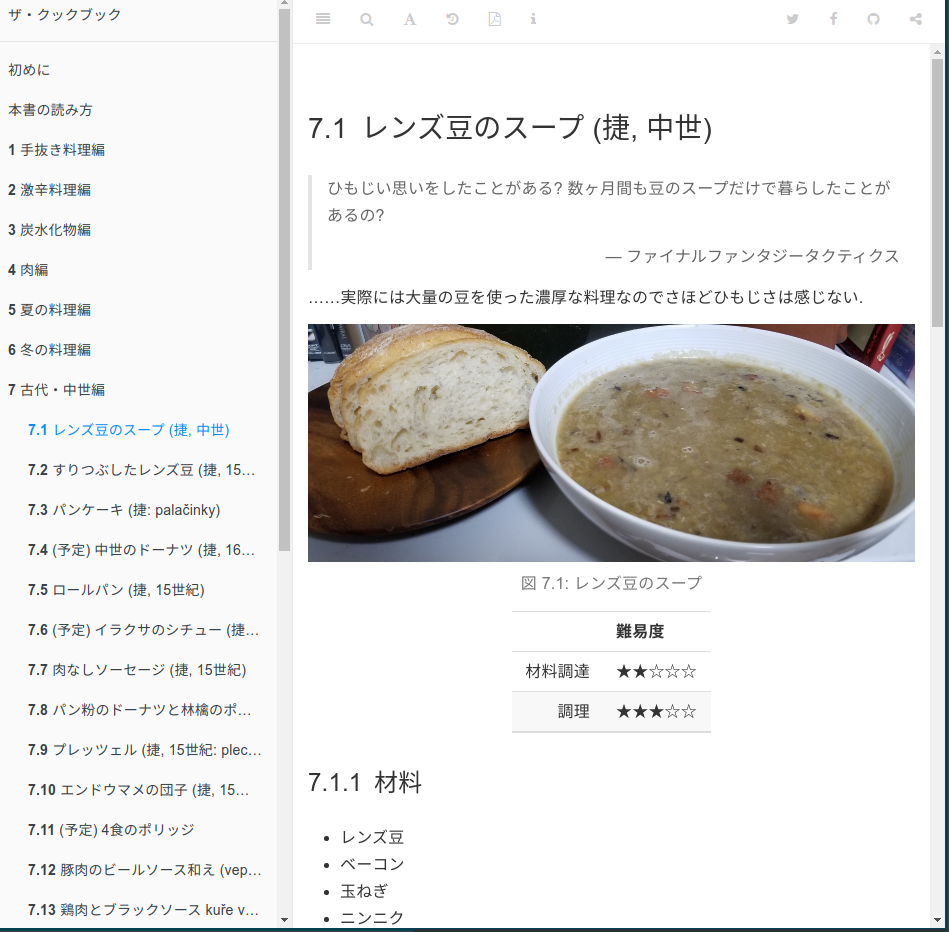
\includegraphics[width=1\linewidth,height=1\textheight,keepaspectratio]{img/cook1} \end{center}
\end{frame}

\hypertarget{r-markdown-ux306eux30cfux30f3ux30baux30aaux30f3ux98a8ux30c1ux30e5ux30fcux30c8ux30eaux30a2ux30eb}{%
\section{R Markdown のハンズオン風チュートリアル}\label{r-markdown-ux306eux30cfux30f3ux30baux30aaux30f3ux98a8ux30c1ux30e5ux30fcux30c8ux30eaux30a2ux30eb}}

\begin{frame}{}
\protect\hypertarget{section}{}
\begin{itemize}
\tightlist
\item
  以降はチュートリアル風に進行
\item
  徐々に高度な機能を使いこなせるようになりましょう
\end{itemize}
\end{frame}

\begin{frame}{最初に用意するもの}
\protect\hypertarget{ux6700ux521dux306bux7528ux610fux3059ux308bux3082ux306e}{}
\begin{itemize}
\tightlist
\item
  OS: Windows 10 or Ubuntu 20.04 or macOS \emph{Catalina}
\item
  最新の R (\textgreater= 4.0.5)\footnote<.->{Windows 以外はあまり気にしなくていい}
\item
  最新の RStudio (\textgreater{} 1.4.11)\footnote<.->{Windows かつ Python 使う人は daily builds}
\item
  rocker で統一してもいいが自分が\sout{面倒がって}使ってないのでマルチプラットフォームで
\end{itemize}
\end{frame}

\begin{frame}[fragile]{必要パッケージ}
\protect\hypertarget{ux5fc5ux8981ux30d1ux30c3ux30b1ux30fcux30b8}{}
\includegraphics[width=\textwidth,height=0.2\textheight]{3ff220644c25a0789576ecaab8ef9934d81a45c0.png}
\includegraphics[width=\textwidth,height=0.2\textheight]{255b9265628fb6b0e920c57406c5343dd9242e3c.png}
\includegraphics[width=\textwidth,height=0.2\textheight]{8b1c73ad9ef1d185900aa4bf322cee34a1f97e6e.png}
\includegraphics[width=\textwidth,height=0.2\textheight]{844ee78a0418bf06133f99513cf48c9ee2a926bf.png}
\includegraphics[width=\textwidth,height=0.2\textheight]{a3abecc912536cfd47b013e781ba83fef54ba4da.png}

\begin{itemize}
\item
  \textbf{rmarkdown}, \textbf{bookdown}, \textbf{remotes}, \textbf{rmdja} パッケージ

  \begin{itemize}
  \tightlist
  \item
    Python を使うなら \textbf{reticulate} も必要
  \end{itemize}

\begin{Shaded}
\begin{Highlighting}[]
\FunctionTok{install.packages}\NormalTok{(}\FunctionTok{c}\NormalTok{(}\StringTok{"rmarkdown"}\NormalTok{, }\StringTok{"bookdown"}\NormalTok{, }\StringTok{"remotes"}\NormalTok{))}
\NormalTok{remotes}\SpecialCharTok{::}\FunctionTok{install\_github}\NormalTok{(}\StringTok{"Gedevan{-}Aleksidze/rmdja"}\NormalTok{)}
\end{Highlighting}
\end{Shaded}
\item
  LaTeX (PDFが必要な場合)

  \begin{itemize}
  \tightlist
  \item
    実インストールなら \textbf{tinytex} パッケージ
  \end{itemize}
\end{itemize}
\end{frame}

\begin{frame}[fragile]{パッケージ等のダウンロード}
\protect\hypertarget{ux30d1ux30c3ux30b1ux30fcux30b8ux7b49ux306eux30c0ux30a6ux30f3ux30edux30fcux30c9}{}
\begin{itemize}
\tightlist
\item
  \href{https://rpubs.com/ktgrstsh/755893}{ここ}に補足資料を上げました.
\item
  \href{https://github.com/Gedevan-Aleksizde/tokyor-91-rmd}{ここ}にソースがあります.
\item
  \texttt{rmd-setup.R} を参考にしてください.
\end{itemize}

\begin{center}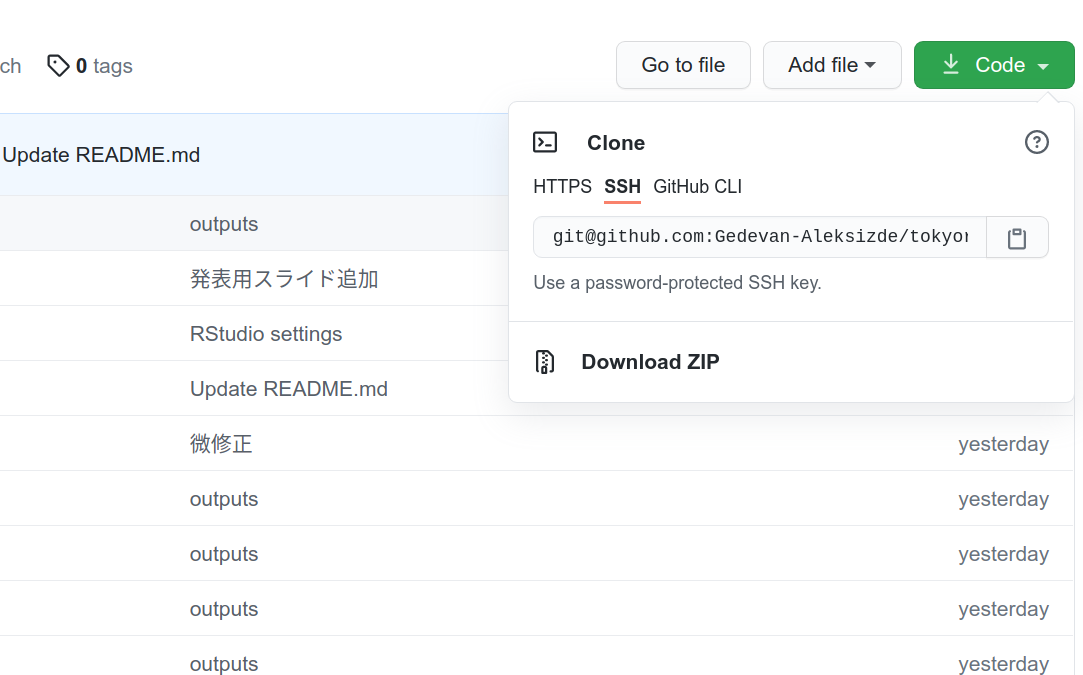
\includegraphics[width=1\linewidth,height=1\textheight,keepaspectratio]{img/github} \end{center}
\end{frame}

\begin{frame}{R Markdown の新規作成 (1/3)}
\protect\hypertarget{r-markdown-ux306eux65b0ux898fux4f5cux6210-13}{}
\begin{enumerate}
\tightlist
\item
  R Markdown\ldots{} を選ぶ
\end{enumerate}

\begin{center}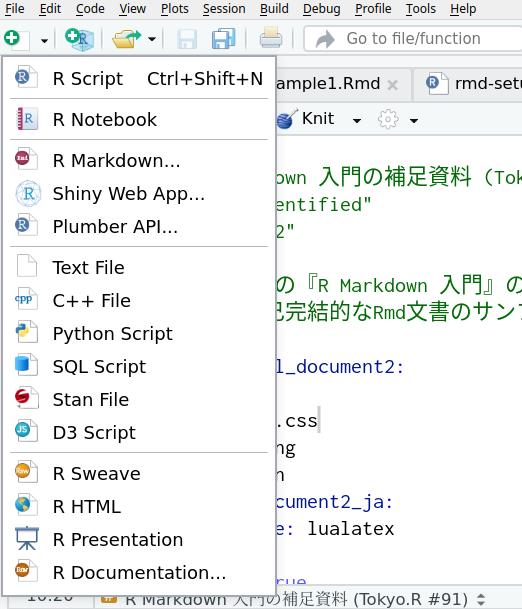
\includegraphics[width=1\linewidth,height=1\textheight,keepaspectratio]{img/newfile} \end{center}
\end{frame}

\begin{frame}{R Markdown の新規作成 (2/3)}
\protect\hypertarget{r-markdown-ux306eux65b0ux898fux4f5cux6210-23}{}
\begin{enumerate}
\setcounter{enumi}{1}
\tightlist
\item
  HTML を選ぶ
\end{enumerate}

\begin{center}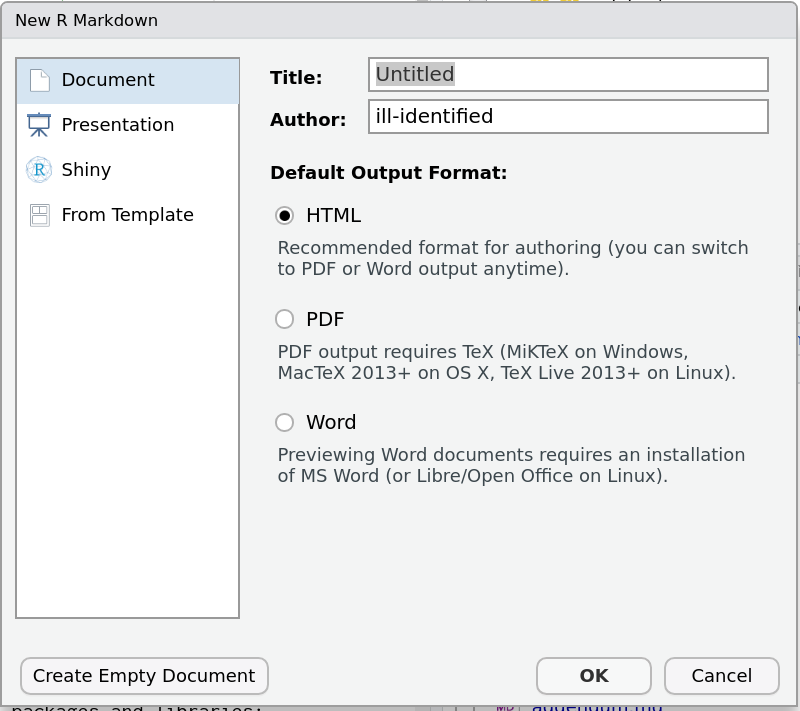
\includegraphics[width=1\linewidth,height=1\textheight,keepaspectratio]{img/select-html} \end{center}
\end{frame}

\begin{frame}[fragile]{R Markdown の新規作成 (3/3)}
\protect\hypertarget{r-markdown-ux306eux65b0ux898fux4f5cux6210-33}{}
\begin{enumerate}
\setcounter{enumi}{2}
\item
  \texttt{title:}, \texttt{author:} を書き換える

  \begin{center}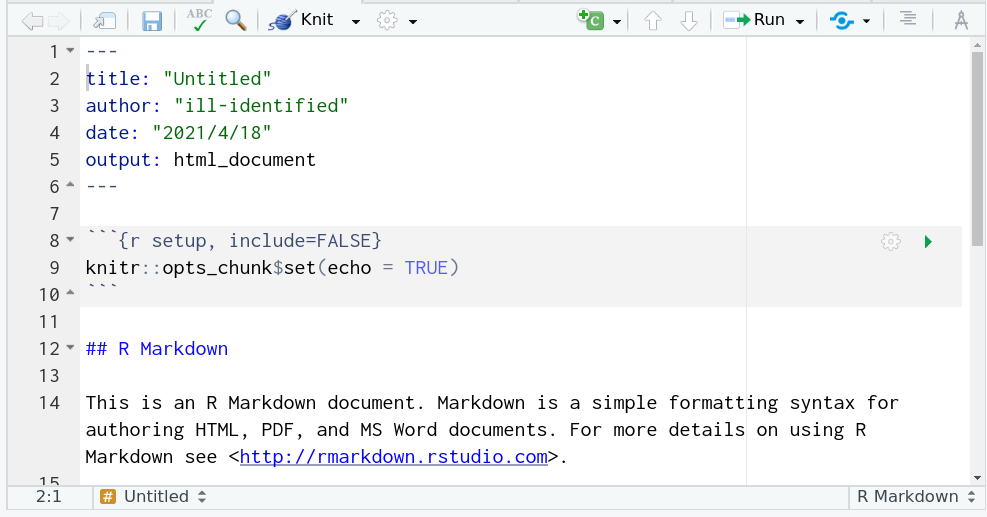
\includegraphics[width=1\linewidth,height=1\textheight,keepaspectratio]{img/newbie} \end{center}
\item
  適当なファイル名で保存
\item
  上の ``Knit'' ボタンでコンパイル
\end{enumerate}
\end{frame}

\begin{frame}{できた!}
\protect\hypertarget{ux3067ux304dux305f}{}
\begin{center}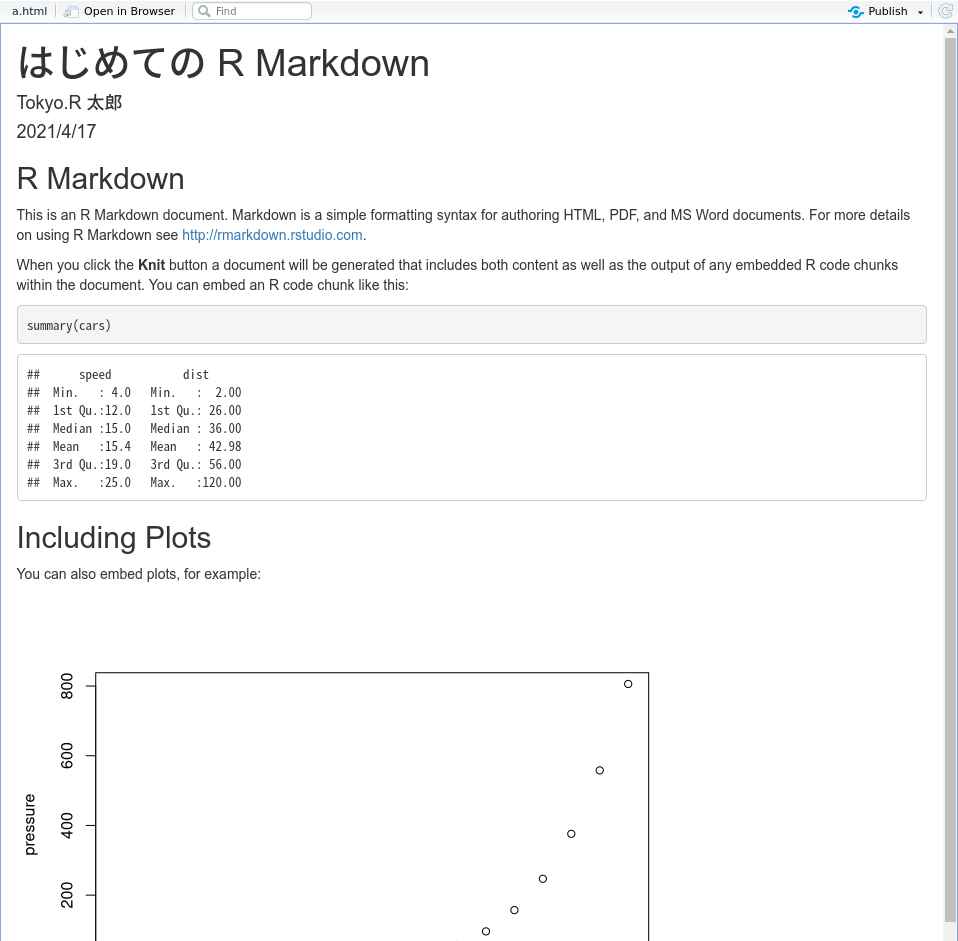
\includegraphics[width=1\linewidth,height=1\textheight,keepaspectratio]{img/plain-document} \end{center}

\ldots{} \textbf{これだけじゃメモ帳と変わらないじゃん!}
\end{frame}

\hypertarget{markdown}{%
\section{Markdown}\label{markdown}}

\begin{frame}{Markdown の基本}
\protect\hypertarget{markdown-ux306eux57faux672c}{}
\begin{itemize}
\item
  Markdown は「マークアップ言語」

  \begin{itemize}
  \tightlist
  \item
    HTMLタグとか, テキストを装飾し,
    「見出し」「段落」など意味を与える
  \end{itemize}
\item
  シンプルなので視覚的に分かりやすい

  \begin{itemize}
  \tightlist
  \item
    HTML のようにタグがゴチャゴチャしてない
  \item
    メモ帳と同じ感覚で使える
  \end{itemize}
\item
  \textbf{方言}が多い点に注意

  \begin{itemize}
  \tightlist
  \item
    例 GitHub, Slack
  \end{itemize}
\end{itemize}
\end{frame}

\begin{frame}[fragile]{Markdown の代表的な構文: 行内要素}
\protect\hypertarget{markdown-ux306eux4ee3ux8868ux7684ux306aux69cbux6587-ux884cux5185ux8981ux7d20}{}
\begin{itemize}
\tightlist
\item
  文のスタイルを部分的に変更する
\end{itemize}

\begin{enumerate}
\item
  文字のスタイル

  \begin{itemize}
  \tightlist
  \item
    「\texttt{**太字**}」 -\textgreater{} 「\textbf{太字}」
  \item
    「\texttt{*斜体/イタリック\ Itacic*}」 -\textgreater{} 「\emph{斜体/イタリック
    Itacic}」\footnote<.->{日本語は対応してないこともある}
  \item
    \texttt{**}/\texttt{*} の代わりに \texttt{\_\_}/\texttt{\_} も可
  \item
    \texttt{1\ +\ 1} (バッククオート) でタイプライタ体 \texttt{1\ +\ 1}
  \item
    「\texttt{\textasciitilde{}\textasciitilde{}打ち消し線\textasciitilde{}\textasciitilde{}}」-\textgreater{} 「\sout{打ち消し線}」
  \end{itemize}
\end{enumerate}
\end{frame}

\begin{frame}[fragile]{Markdown の代表的な構文: 行内数式}
\protect\hypertarget{markdown-ux306eux4ee3ux8868ux7684ux306aux69cbux6587-ux884cux5185ux6570ux5f0f}{}
\begin{enumerate}
\setcounter{enumi}{1}
\item
  LaTeX 数式

  \begin{itemize}
  \tightlist
  \item
    「\texttt{\$f(x)\$}」 -\textgreater{} 「\(f(x)\)」
  \end{itemize}
\item
  独立行なら \texttt{\$\$} で囲む

  \begin{itemize}
  \tightlist
  \item
    または, \texttt{align} など直接 LaTeX を書く
  \end{itemize}
\end{enumerate}
\end{frame}

\begin{frame}[fragile]{Markdown の代表的な構文: ブロック要素 (1/2)}
\protect\hypertarget{markdown-ux306eux4ee3ux8868ux7684ux306aux69cbux6587-ux30d6ux30edux30c3ux30afux8981ux7d20-12}{}
\begin{itemize}
\tightlist
\item
  テキストのまとまりを定義する
\end{itemize}

\begin{enumerate}
\item
  行頭に「\texttt{\#}」で見出し \texttt{\#\ 第1章:\ 序}

  \begin{itemize}
  \tightlist
  \item
    \texttt{\#} を増やすと階層が深くなる
  \item
    このスライドのタイトルは \texttt{\#\#}
  \end{itemize}
\item
  行頭に「\texttt{*}」で箇条書き

  \begin{itemize}
  \tightlist
  \item
    直後のスペース必須
  \item
    インデントで階層化可能
  \item
    インデントは \textbf{tab 2個} (スペース4つ) 以上\footnote<.->{RStudio のデフォルト設定のため}
  \end{itemize}
\item
  「\texttt{1.}」 or 「\texttt{a.}」で番号付き箇条書き

  \begin{enumerate}
  [a.]
  \tightlist
  \item
    これもインデント可
  \item
    番号を書かなくても\textbf{自動で調整}
  \end{enumerate}
\end{enumerate}
\end{frame}

\begin{frame}[fragile]{Markdown の代表的な構文: ブロック要素 (2/2)}
\protect\hypertarget{markdown-ux306eux4ee3ux8868ux7684ux306aux69cbux6587-ux30d6ux30edux30c3ux30afux8981ux7d20-22}{}
\begin{enumerate}
\setcounter{enumi}{3}
\item
  コメントアウトは HTML 方式 \texttt{\textless{}!-\/-\ ここは出力されない\ -\/-\textgreater{}}
\item
  見出しブロック (Beamer のみ)
\end{enumerate}

\begin{alertblock}{これは警告です}
これは \texttt{alertblock} 環境

\end{alertblock}

\begin{itemize}
\tightlist
\item
  表を記述することもできるが省略
\item
  わかりにくかったらこのスライドの Rmd ファイルで見てね
\end{itemize}
\end{frame}

\begin{frame}{Visual Markdown Editor}
\protect\hypertarget{visual-markdown-editor}{}
\begin{itemize}
\tightlist
\item
  どうしても苦手なら Word のような編集モードあり
\item
  右上のコンパスマークをクリック
\end{itemize}

\begin{center}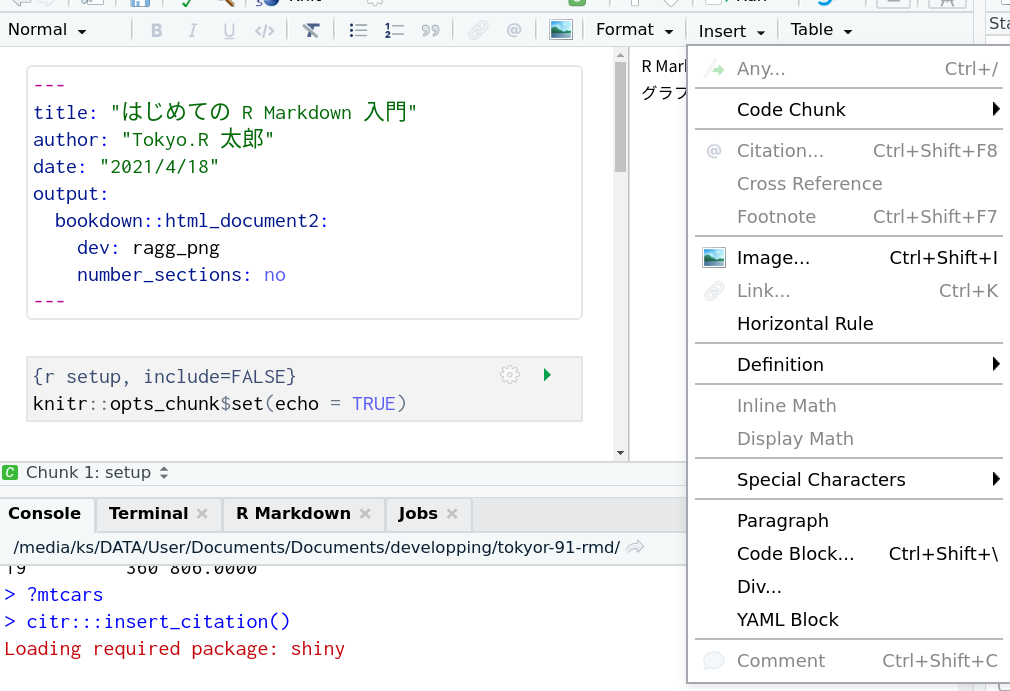
\includegraphics[width=1\linewidth,height=1\textheight,keepaspectratio]{img/visual-editor1} \end{center}

\begin{center}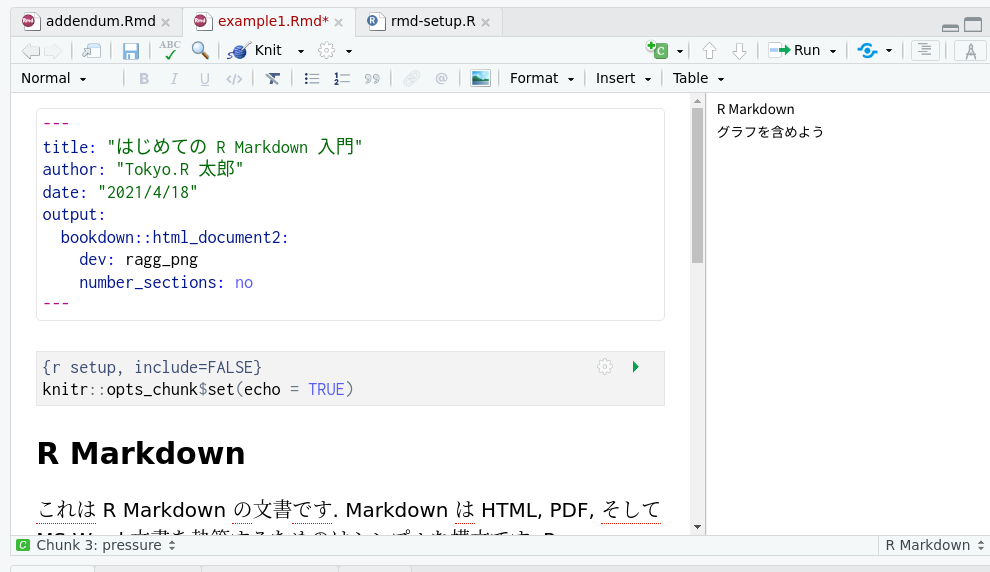
\includegraphics[width=1\linewidth,height=1\textheight,keepaspectratio]{img/visual-editor2} \end{center}
\end{frame}

\hypertarget{r-ux30b3ux30fcux30c9ux306eux57cbux3081ux8fbcux307f}{%
\section{R コードの埋め込み}\label{r-ux30b3ux30fcux30c9ux306eux57cbux3081ux8fbcux307f}}

\begin{frame}[fragile]{コードチャンクと行内コード}
\protect\hypertarget{ux30b3ux30fcux30c9ux30c1ux30e3ux30f3ux30afux3068ux884cux5185ux30b3ux30fcux30c9}{}
\begin{itemize}
\tightlist
\item
  R コードの埋め込みは2種類
\item
  独立したブロックとしてのコードチャンク

  \begin{itemize}
  \tightlist
  \item
    表やグラフの埋め込み
  \item
    ソースコードの掲載
  \item
    その他複雑な処理
  \item
    他のプログラミング言語も使用可能
  \end{itemize}
\item
  簡単な1文だけのコードの行内埋め込み

  \begin{itemize}
  \tightlist
  \item
    1 + 1 = 2 のように Markdown 内に出力を埋め込める
  \item
    「2」の部分は実際には \texttt{\textasciigrave{}r\ 1\ +\ 1\textasciigrave{}}
    と書いている
  \end{itemize}
\end{itemize}
\end{frame}

\begin{frame}[fragile]{行内コード}
\protect\hypertarget{ux884cux5185ux30b3ux30fcux30c9}{}
\begin{itemize}
\item
  \texttt{\textasciigrave{}r\ \textless{}R\ コード\textgreater{}\textasciigrave{}}
\item
  複雑なコードは書けない

  \begin{itemize}
  \tightlist
  \item
    単文でできることのみ
  \end{itemize}
\item
  原則文字の出力のみ

  \begin{itemize}
  \tightlist
  \item
    グラフや表は想定されていない
  \end{itemize}
\item
  よくある使い方

  \begin{itemize}
  \tightlist
  \item
    表紙の日付を自動更新
  \item
    \texttt{date:\ 2021-04-17}
  \end{itemize}
\end{itemize}
\end{frame}

\begin{frame}[fragile]{コードチャンク (1/2)}
\protect\hypertarget{ux30b3ux30fcux30c9ux30c1ux30e3ux30f3ux30af-12}{}
\begin{itemize}
\tightlist
\item
  より複雑なプログラムを書き, 図表を出力できる
\end{itemize}

\begin{verbatim}
```{r, LABEL, echo=T}
1 + 1
summary(mtcars)
```
\end{verbatim}

\begin{itemize}
\tightlist
\item
  LABEL は自由な名前を付けてよい

  \begin{itemize}
  \tightlist
  \item
    省略してもよい
  \end{itemize}
\item
  それ以降は「チャンクオプション」

  \begin{itemize}
  \tightlist
  \item
    出力結果などを制御する
  \item
    R の引数と同じように書ける
  \end{itemize}
\end{itemize}
\end{frame}

\begin{frame}{コードチャンク (2/2)}
\protect\hypertarget{ux30b3ux30fcux30c9ux30c1ux30e3ux30f3ux30af-22}{}
\begin{itemize}
\tightlist
\item
  作業中の実行も可能
\item
  右の矢印をクリック
\item
  R notebook を使うのもあり
\end{itemize}

\begin{center}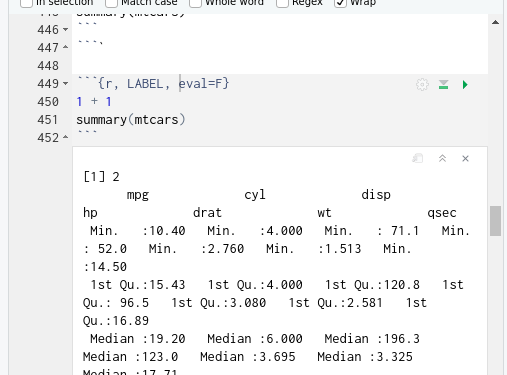
\includegraphics[width=1\linewidth,height=1\textheight,keepaspectratio]{img/knitr} \end{center}
\end{frame}

\begin{frame}[fragile]{よく使うチャンクオプション}
\protect\hypertarget{ux3088ux304fux4f7fux3046ux30c1ux30e3ux30f3ux30afux30aaux30d7ux30b7ux30e7ux30f3}{}
\begin{itemize}
\item
  \texttt{echo}: コードを表示するかどうか

  \begin{itemize}
  \tightlist
  \item
    スライドでは邪魔なのでよく非表示にする
  \end{itemize}
\item
  \texttt{eval=F}: コードを実行しない

  \begin{itemize}
  \tightlist
  \item
    コードだけ見せたい時に
  \end{itemize}
\item
  \texttt{fig.cap=""}: 図のキャプション
\item
  詳細は \href{https://gedevan-aleksizde.github.io/knitr-doc-ja/index.html}{ここ} とか参照
\end{itemize}
\end{frame}

\hypertarget{htmlpdfdocxpptx-ux3078ux306eux5909ux63db}{%
\section{HTML/PDF/DOCX/PPTX への変換}\label{htmlpdfdocxpptx-ux3078ux306eux5909ux63db}}

\begin{frame}{HTML/PDF/DOCX/PPTX への変換}
\begin{itemize}
\tightlist
\item
  HTML はすでにやった通り
\item
  ドキュメントの出力をかえるには \textbf{YAML メタデータ}を書き換える
\item
  PDF/DOCX (Word)/PPTX (パワポ) はちょっと複雑
\item
  というか異なるフォーマットの同時出力が複雑
\end{itemize}
\end{frame}

\begin{frame}[fragile]{出力フォーマット関数}
\protect\hypertarget{ux51faux529bux30d5ux30a9ux30fcux30deux30c3ux30c8ux95a2ux6570}{}
\begin{itemize}
\tightlist
\item
  出力フォーマットが主に文書の体裁を決める
\item
  \texttt{output:\ html\_document} の部分で指定
\item
  \textbf{rmarkdown} にいくつも用意されている
\item
  しかし実際には他のパッケージのほうが便利
\end{itemize}

\begin{table}
\centering
\resizebox{\linewidth}{!}{
\begin{tabular}[t]{l>{}l>{}l}
\toprule
ファイル形式 & デフォルト & おすすめ\\
\midrule
\cellcolor{gray!6}{PDF} & \ttfamily{\cellcolor{gray!6}{pdf\_document}} & \ttfamily{\cellcolor{gray!6}{rmdja::pdf\_document2\_ja}}\\
HTML & \ttfamily{html\_document} & \ttfamily{bookdown::html\_document2}\\
\cellcolor{gray!6}{Word (DOCX)} & \ttfamily{\cellcolor{gray!6}{word\_document}} & \ttfamily{\cellcolor{gray!6}{officedown::rdocx\_document}}\\
スライド (PDF) & \ttfamily{beamer\_presentation} & \ttfamily{rmdja::beamer\_presentation\_ja}\\
\cellcolor{gray!6}{スライド (HTML)} & \ttfamily{\cellcolor{gray!6}{slidy\_presentation}} & \ttfamily{\cellcolor{gray!6}{?}}\\
スライド (PPTX) & \ttfamily{powerpoint\_presentation} & \ttfamily{officedown::rpptx\_document}\\
\bottomrule
\end{tabular}}
\end{table}
\end{frame}

\begin{frame}[fragile]{PDF の設定}
\protect\hypertarget{pdf-ux306eux8a2dux5b9a}{}
最小限の設定はこうだが\ldots{}

\begin{Shaded}
\begin{Highlighting}[]
\FunctionTok{output}\KeywordTok{:}
\AttributeTok{  }\FunctionTok{pdf\_document}\KeywordTok{:}
\AttributeTok{    }\FunctionTok{latex\_engine}\KeywordTok{:}\AttributeTok{ lualatex}
\FunctionTok{documentclass}\KeywordTok{:}\AttributeTok{ ltjsarticle}
\FunctionTok{classoption}\KeywordTok{:}\AttributeTok{ haranoaji}
\end{Highlighting}
\end{Shaded}
\end{frame}

\begin{frame}{まずうまくいかない}
\protect\hypertarget{ux307eux305aux3046ux307eux304fux3044ux304bux306aux3044}{}
\begin{itemize}
\item
  実際に使うといろいろとボロが出ます

  \begin{itemize}
  \tightlist
  \item
    打ち消し線を使うとエラー
  \item
    参考文献リストが変
  \item
    存在しないフォントは使えない
  \end{itemize}
\end{itemize}
\end{frame}

\begin{frame}{PDF は \textbf{rmdja} を使え (1/3)}
\protect\hypertarget{pdf-ux306f-rmdja-ux3092ux4f7fux3048-13}{}
\begin{itemize}
\item
  PDF が難しい理由

  \begin{enumerate}
  \tightlist
  \item
    デフォルト設定が日本語を想定していないため
  \item
    LaTeX の設定も意識する必要
  \item
    HTML と比べるとデフォルトの見た目が寂しい
  \item
    そもそも用途が HTML と違う
  \end{enumerate}
\item
  PDFをHTMLと両立して日本語出力するため \href{https://github.com/Gedevan-Aleksizde/rmdja}{\textbf{rmdja}} を作った

  \begin{itemize}
  \tightlist
  \item
    インストール方法は\href{https://rpubs.com/ktgrstsh/755893}{参考資料}の通り
  \end{itemize}
\end{itemize}
\end{frame}

\begin{frame}{PDF は \textbf{rmdja} を使え (2/3)}
\protect\hypertarget{pdf-ux306f-rmdja-ux3092ux4f7fux3048-23}{}
\begin{itemize}
\tightlist
\item
  まずはインストール
\item
  テンプレートから選ぶ
\end{itemize}

\begin{center}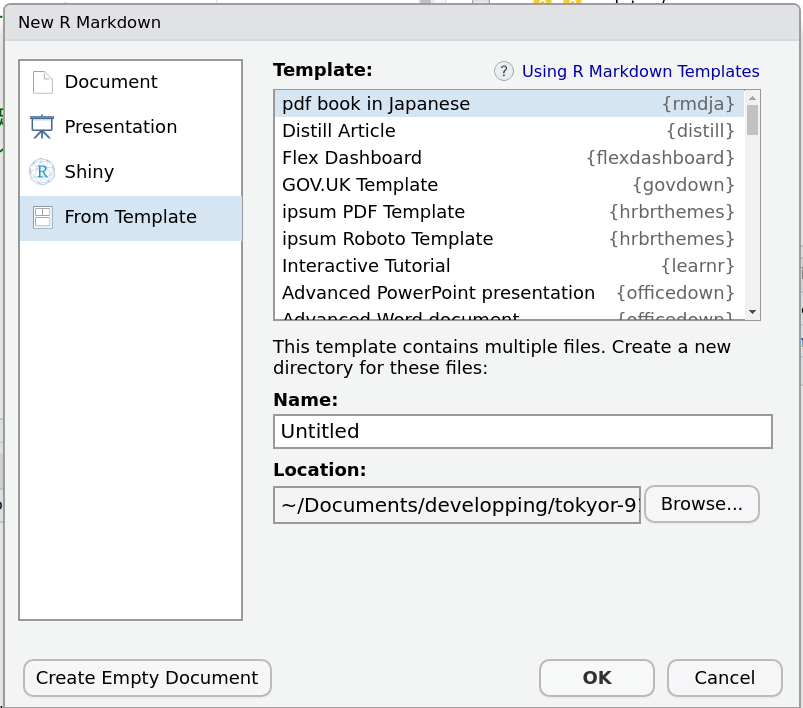
\includegraphics[width=1\linewidth,height=1\textheight,keepaspectratio]{img/templates} \end{center}
\end{frame}

\begin{frame}{PDF は \textbf{rmdja} を使え (3/3)}
\protect\hypertarget{pdf-ux306f-rmdja-ux3092ux4f7fux3048-33}{}
\begin{itemize}
\tightlist
\item
  もともとはスライド作成用だった
\item
  現在は HTML/PDFの出力を両立できること目指す
\item
  現在は以下の4種類の PDF フォーマット
\end{itemize}

\begin{enumerate}
\tightlist
\item
  書籍
\item
  論文
\item
  スライド
\item
  縦書き
\end{enumerate}
\end{frame}

\begin{frame}[fragile]{Word への出力 (1/2)}
\protect\hypertarget{word-ux3078ux306eux51faux529b-12}{}
\begin{itemize}
\tightlist
\item
  最低限の設定
\end{itemize}

\begin{Shaded}
\begin{Highlighting}[]
\FunctionTok{output}\KeywordTok{:}\AttributeTok{ word\_document}
\end{Highlighting}
\end{Shaded}

\begin{center}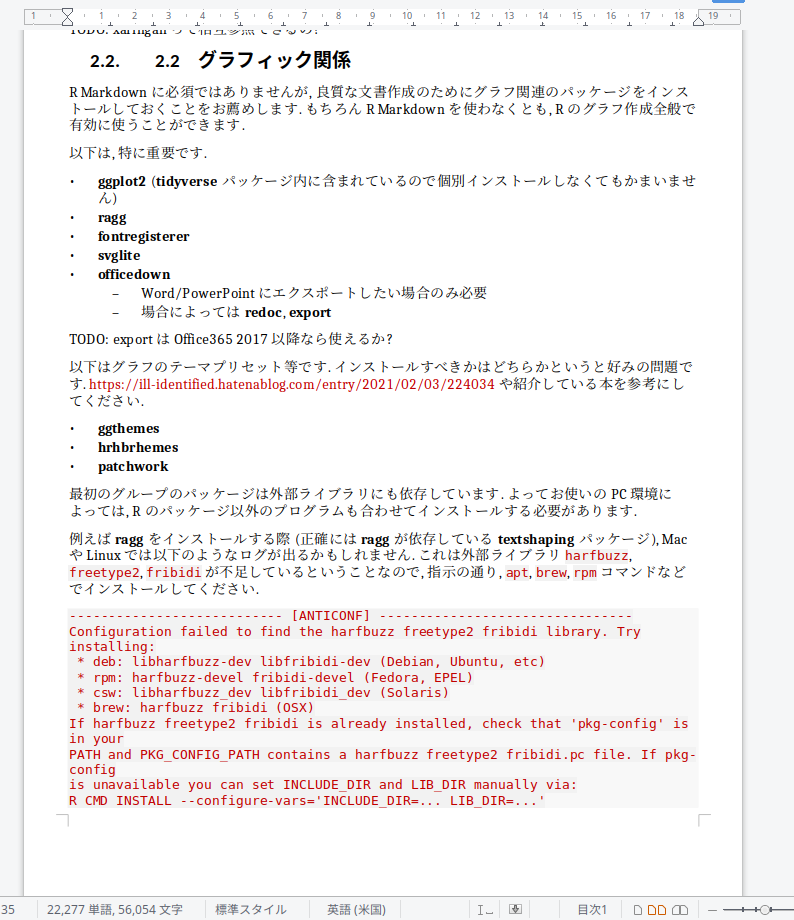
\includegraphics[width=1\linewidth,height=1\textheight,keepaspectratio]{img/libre} \end{center}
\end{frame}

\begin{frame}[fragile]{Word への出力 (2/2)}
\protect\hypertarget{word-ux3078ux306eux51faux529b-22}{}
\begin{itemize}
\tightlist
\item
  おすすめ
\item
  (たまにうまく行かないことがある)
\end{itemize}

\begin{Shaded}
\begin{Highlighting}[]
\FunctionTok{output}\KeywordTok{:}\AttributeTok{ officedown::rdocx\_document:}
\AttributeTok{  }\FunctionTok{base\_format}\KeywordTok{:}\AttributeTok{ bookdown::word\_document2}
\AttributeTok{  }\FunctionTok{toc}\KeywordTok{:}\AttributeTok{ }\CharTok{true}
\AttributeTok{    }\FunctionTok{tables}\KeywordTok{:}
\AttributeTok{      }\FunctionTok{caption}\KeywordTok{:}
\AttributeTok{        }\FunctionTok{pre}\KeywordTok{:}\AttributeTok{ }\StringTok{"表"}
\AttributeTok{    }\FunctionTok{plots}\KeywordTok{:}
\AttributeTok{      }\FunctionTok{style}\KeywordTok{:}
\AttributeTok{        }\FunctionTok{aling}\KeywordTok{:}\AttributeTok{ center}
\AttributeTok{      }\FunctionTok{caption}\KeywordTok{:}
\AttributeTok{        }\FunctionTok{pre}\KeywordTok{:}\AttributeTok{ }\StringTok{"図"}
\end{Highlighting}
\end{Shaded}
\end{frame}

\begin{frame}{Word への出力 (3/2)}
\protect\hypertarget{word-ux3078ux306eux51faux529b-32}{}
\begin{itemize}
\item
  (余計なお世話?) 本当に Word を使う必要がある?

  \begin{itemize}
  \tightlist
  \item
    提出物はHTMLやPDFじゃダメ?
  \item
    共著者がWordしか使えない?
  \end{itemize}
\item
  RMD は PDF を直接作れます
\end{itemize}
\end{frame}

\begin{frame}[fragile]{パワーポイントへの出力 (PPTX)}
\protect\hypertarget{ux30d1ux30efux30fcux30ddux30a4ux30f3ux30c8ux3078ux306eux51faux529b-pptx}{}
\begin{itemize}
\tightlist
\item
  \sout{あんまり使ってないけどたぶんいける}
\end{itemize}

\begin{Shaded}
\begin{Highlighting}[]
\FunctionTok{output}\KeywordTok{:}\AttributeTok{ powerpoint\_presentation}
\end{Highlighting}
\end{Shaded}

\begin{Shaded}
\begin{Highlighting}[]
\FunctionTok{output}\KeywordTok{:}\AttributeTok{ officedown::rpptx\_presentation}
\end{Highlighting}
\end{Shaded}

\begin{center}
\includegraphics[width=1\linewidth,height=1\textheight,keepaspectratio]{img/powerpoint} \end{center}
\end{frame}

\begin{frame}[fragile]{スライドへの出力 (PDF)}
\protect\hypertarget{ux30b9ux30e9ux30a4ux30c9ux3078ux306eux51faux529b-pdf}{}
\begin{itemize}
\tightlist
\item
  最も簡単な方法
\item
  \textbf{rmdja} パッケージのほうが便利です (たぶん)
\end{itemize}

\begin{Shaded}
\begin{Highlighting}[]
\FunctionTok{output}\KeywordTok{:}
\AttributeTok{  }\FunctionTok{beamer\_presentation}\KeywordTok{:}
\AttributeTok{    }\FunctionTok{latex\_engine}\KeywordTok{:}\AttributeTok{ lualatex}
\FunctionTok{mainfont}\KeywordTok{:}\AttributeTok{ haranoaji}
\end{Highlighting}
\end{Shaded}
\end{frame}

\begin{frame}{Q.: スライドからはみ出すんだけど?}
\protect\hypertarget{q.-ux30b9ux30e9ux30a4ux30c9ux304bux3089ux306fux307fux51faux3059ux3093ux3060ux3051ux3069}{}
\begin{itemize}
\tightlist
\item
  A.: 慣れましょう
\item
  詰め込み過ぎは良くないです
\item
  \sout{この発表みたいになります}
\end{itemize}
\end{frame}

\begin{frame}[fragile]{YAML について}
\protect\hypertarget{yaml-ux306bux3064ux3044ux3066}{}
\begin{itemize}
\tightlist
\item
  \texttt{title:}, \texttt{author}, \texttt{output:} は \textbf{YAML メタデータ}と呼ばれる
\item
  カスタマイズに重要
\item
  細かい話になるので冒頭の\href{https://rpubs.com/ktgrstsh/755893}{資料}を見てください
\end{itemize}
\end{frame}

\hypertarget{ux3061ux3087ux3063ux3068ux767aux5c55ux7684ux306aux8a71}{%
\section{ちょっと発展的な話}\label{ux3061ux3087ux3063ux3068ux767aux5c55ux7684ux306aux8a71}}

\begin{frame}[fragile]{相互参照}
\protect\hypertarget{ux76f8ux4e92ux53c2ux7167}{}
\begin{itemize}
\item
  図・表・セクション見出し, 数式, 引用文献を参照したい
\item
  「図1が分析結果である」「2章を見よ」など文書内の参照
\item
  番号やハイパーリンクを自分で書くと後で修正するのが大変
\item
  \textbf{bookdown} 系のフォーマットで実現

  \begin{itemize}
  \tightlist
  \item
    \textbf{rmarkdown} 単体では不可
  \item
    末尾に \texttt{2} と付くフォーマット
  \end{itemize}
\end{itemize}
\end{frame}

\begin{frame}[fragile]{図・画像への相互参照}
\protect\hypertarget{ux56f3ux753bux50cfux3078ux306eux76f8ux4e92ux53c2ux7167}{}
\begin{itemize}
\item
  コードチャンクへ参照する形で実現

  \begin{itemize}
  \tightlist
  \item
    画像ファイルは \texttt{knitr::include\_graphics()}
  \end{itemize}
\end{itemize}

\begin{enumerate}
\tightlist
\item
  コードチャンクのラベルを書く
\item
  \texttt{fig.cap="キャプション"} オプションでキャプションを書く
\item
  \texttt{\textbackslash{}@ref(fig:チャンクラベル)} で参照
\end{enumerate}
\end{frame}

\begin{frame}[fragile]{画像への相互参照の実例}
\protect\hypertarget{ux753bux50cfux3078ux306eux76f8ux4e92ux53c2ux7167ux306eux5b9fux4f8b}{}
\begin{itemize}
\tightlist
\item
  図\ref{fig:image1} を見よ!
\item
  \textbf{ggplot2} ももちろん掲載できる
\end{itemize}

\texttt{\{r,\ image1,\ fig.cap="図への相互参照"\}\ knitr::include\_graphics("img/logo.png")}

\begin{figure}

{\centering 
\includegraphics[width=1\linewidth,height=0.3\textheight,keepaspectratio]{img/logo} 

}

\caption{図への相互参照}\label{fig:image1}
\end{figure}
\end{frame}

\begin{frame}[fragile]{表への相互参照}
\protect\hypertarget{ux8868ux3078ux306eux76f8ux4e92ux53c2ux7167}{}
\begin{itemize}
\item
  データフレームをそのまま表にできる
\item
  チャンクラベルを指定
\item
  \texttt{knitr::kable(df,\ caption="...")} が表のスタイルを自動生成

  \begin{itemize}
  \tightlist
  \item
    チャンクオプションではないことに注意
  \end{itemize}
\item
  \texttt{\textbackslash{}@ref(tab:チャンクラベル)} というふうに指定
\end{itemize}
\end{frame}

\begin{frame}[fragile]{表への相互参照の実例}
\protect\hypertarget{ux8868ux3078ux306eux76f8ux4e92ux53c2ux7167ux306eux5b9fux4f8b}{}
\begin{itemize}
\tightlist
\item
  \textbf{kableExtra} による表\ref{tab:table1}を見よ!!
\end{itemize}

\begin{verbatim}
```{r, table1}
knitr::kable(head(mtcars, 4),
             caption="表への相互参照")`
```
\end{verbatim}

\begin{table}

\caption{\label{tab:table1}表への相互参照}
\centering
\resizebox{\linewidth}{!}{
\begin{tabular}[t]{lrrrrrrrrrrr}
\toprule
  & mpg & cyl & disp & hp & drat & wt & qsec & vs & am & gear & carb\\
\midrule
\cellcolor{gray!6}{Mazda RX4} & \cellcolor{gray!6}{21.0} & \cellcolor{gray!6}{6} & \cellcolor{gray!6}{160} & \cellcolor{gray!6}{110} & \cellcolor{gray!6}{3.90} & \cellcolor{gray!6}{2.620} & \cellcolor{gray!6}{16.46} & \cellcolor{gray!6}{0} & \cellcolor{gray!6}{1} & \cellcolor{gray!6}{4} & \cellcolor{gray!6}{4}\\
Mazda RX4 Wag & 21.0 & 6 & 160 & 110 & 3.90 & 2.875 & 17.02 & 0 & 1 & 4 & 4\\
\cellcolor{gray!6}{Datsun 710} & \cellcolor{gray!6}{22.8} & \cellcolor{gray!6}{4} & \cellcolor{gray!6}{108} & \cellcolor{gray!6}{93} & \cellcolor{gray!6}{3.85} & \cellcolor{gray!6}{2.320} & \cellcolor{gray!6}{18.61} & \cellcolor{gray!6}{1} & \cellcolor{gray!6}{1} & \cellcolor{gray!6}{4} & \cellcolor{gray!6}{1}\\
Hornet 4 Drive & 21.4 & 6 & 258 & 110 & 3.08 & 3.215 & 19.44 & 1 & 0 & 3 & 1\\
\bottomrule
\end{tabular}}
\end{table}
\end{frame}

\begin{frame}[fragile]{相互参照のさらなる応用}
\protect\hypertarget{ux76f8ux4e92ux53c2ux7167ux306eux3055ux3089ux306aux308bux5fdcux7528}{}
\begin{itemize}
\item
  複数の図表を1つにまとめることも可能

  \begin{itemize}
  \tightlist
  \item
    詳細は Cookbook
  \end{itemize}
\item
  引用文献のスタイル変更

  \begin{itemize}
  \tightlist
  \item
    PDF は BibLaTeX (\texttt{.bbx})
  \item
    HTML は CSL (\texttt{.csl})
  \item
    (u)pBibTeX (\texttt{.bst}) はちょっとややこしい
  \end{itemize}
\item
  論文フォーマットは LaTeX に依存している事が多いので一般化は難しい
\end{itemize}
\end{frame}

\begin{frame}[fragile]{R 以外の言語}
\protect\hypertarget{r-ux4ee5ux5916ux306eux8a00ux8a9e}{}
\begin{itemize}
\item
  コードチャンクには R 以外の言語も使える

  \begin{itemize}
  \tightlist
  \item
    \texttt{r} を別の言語に書き換える
  \item
    \texttt{stan} コードを直接書くことも可能
  \end{itemize}
\item
  Python, Julia も同様に使える

  \begin{itemize}
  \tightlist
  \item
    それ以外は別のチャンクに設定・変数を持ち越せない
  \item
    チャンクごとにプログラムを呼び出しているため
  \end{itemize}
\item
  Python 使用例: 例のスライド
\item
  新規登録も可能
\item
  詳細はクックブック15章
\end{itemize}
\end{frame}

\begin{frame}[fragile]{Python のコードチャンク}
\protect\hypertarget{python-ux306eux30b3ux30fcux30c9ux30c1ux30e3ux30f3ux30af}{}
\begin{itemize}
\tightlist
\item
  \textbf{reticulate} パッケージで使用可能
\item
  RStudio 1.4 からかなり使いやすくなった
\item
  コードチャンクの \texttt{r} の部分を \texttt{python} に
\end{itemize}

\begin{Shaded}
\begin{Highlighting}[]
\ImportTok{import}\NormalTok{ numpy }\ImportTok{as}\NormalTok{ np}
\NormalTok{np.array([}\DecValTok{1}\NormalTok{, }\DecValTok{1}\NormalTok{])}
\end{Highlighting}
\end{Shaded}

\begin{verbatim}
array([1, 1])
\end{verbatim}
\end{frame}

\begin{frame}[fragile]{Julia のコードチャンク}
\protect\hypertarget{julia-ux306eux30b3ux30fcux30c9ux30c1ux30e3ux30f3ux30af}{}
\begin{itemize}
\tightlist
\item
  \textbf{JuliaCall} パッケージで使用可能
\item
  \url{https://julialang.org/downloads/}
\item
  まだ不安定なところが多い
\item
  古いバージョンにする必要
\item
  Gadfly が使えない?
\item
  画像の保存は手動にしたほうが安定?
\item
  参考: \href{https://github.com/piever/Remark.jl}{\texttt{Remark.jl}} という Julia パッケージあり

  \begin{itemize}
  \tightlist
  \item
    \texttt{remark.js} ベース
  \end{itemize}
\end{itemize}
\end{frame}

\begin{frame}[fragile]{Julia 使用例 (失敗!!)}
\protect\hypertarget{julia-ux4f7fux7528ux4f8b-ux5931ux6557}{}
\begin{itemize}
\tightlist
\item
  要 Julia 本体 \& \textbf{JuliaCall} \& 環境設定
\end{itemize}

\begin{Shaded}
\begin{Highlighting}[]
\KeywordTok{using}\NormalTok{ Plots}
\NormalTok{gr()}
\end{Highlighting}
\end{Shaded}

\begin{verbatim}
Plots.GRBackend()
\end{verbatim}

\begin{Shaded}
\begin{Highlighting}[]
\NormalTok{plot(Plots.fakedata(}\FloatTok{50}\OperatorTok{,}\FloatTok{5}\NormalTok{)}\OperatorTok{,}\NormalTok{w}\OperatorTok{=}\FloatTok{3}\NormalTok{)}
\end{Highlighting}
\end{Shaded}

\begin{verbatim}
Plot{Plots.GRBackend() n=5}
\end{verbatim}
\end{frame}

\hypertarget{pdflatex-ux95a2ux4fc2ux306eux5fdcux7528}{%
\section{PDF/LaTeX 関係の応用}\label{pdflatex-ux95a2ux4fc2ux306eux5fdcux7528}}

\begin{frame}[fragile]{PDF/LaTeX 周りの予備知識}
\protect\hypertarget{pdflatex-ux5468ux308aux306eux4e88ux5099ux77e5ux8b58}{}
\begin{itemize}
\item
  PDF は LaTeX を使用して生成

  \begin{itemize}
  \tightlist
  \item
    いくつかのエンジンがある
  \end{itemize}
\item
  文書全体のスタイルは主に LaTeX の文書クラスファイルで定義

  \begin{itemize}
  \tightlist
  \item
    \texttt{bxjsarticle}, \texttt{ltjsarticle}, \texttt{beamer}, etc.
  \end{itemize}
\end{itemize}
\end{frame}

\begin{frame}[fragile]{どの LaTeX エンジンを使うべきか}
\protect\hypertarget{ux3069ux306e-latex-ux30a8ux30f3ux30b8ux30f3ux3092ux4f7fux3046ux3079ux304dux304b}{}
\begin{itemize}
\item
  \texttt{latex\_engine} でエンジンを変更できる
\item
  \textbf{結論}: 詳しくない人は \texttt{xelatex}
  (\XeLaTeX)/\texttt{lualatex}
  (\LuaLaTeX) 2択
\item
  \XeLaTeX: 禁則処理に一部\textbf{難あり}, 速い

  \begin{itemize}
  \tightlist
  \item
    スライドだと気にならない?
  \end{itemize}
\item
  \LuaLaTeX: 使用者が多い, \textbf{遅い}
\item
  \pdfLaTeX: 日本語メインなら\textbf{使わない}

  \begin{itemize}
  \tightlist
  \item
    欧文ジャーナルでは現役
  \end{itemize}
\item
  \pLaTeX, \upLaTeX -\textgreater{} Rmd
  の\textbf{サポート外}

  \begin{itemize}
  \tightlist
  \item
    後述
  \end{itemize}
\end{itemize}
\end{frame}

\begin{frame}{}
\protect\hypertarget{section-1}{}
以降は詳しい人 or 詳しくなることを強いられている人向け
\end{frame}

\begin{frame}[fragile]{Rmd のサポート外の処理}
\protect\hypertarget{rmd-ux306eux30b5ux30ddux30fcux30c8ux5916ux306eux51e6ux7406}{}
\begin{itemize}
\item
  以下を要求する国内学会公式フォーマット

  \begin{itemize}
  \tightlist
  \item
    (u)\pLaTeX 前提の \texttt{.cls}/\texttt{.sty}
  \item
    (u)\pBibTeX 前提の \texttt{.bst}
  \end{itemize}
\item
  いずれも\textbf{デフォルトの Rmd では非対応}

  \begin{itemize}
  \tightlist
  \item
    日本独自開発の処理系のため
  \end{itemize}
\item
  要 \textbf{tinytex} のエミュレーション無効化

  \begin{itemize}
  \tightlist
  \item
    以下をチャンクのどこかに書く
  \end{itemize}

\begin{Shaded}
\begin{Highlighting}[]
\FunctionTok{options}\NormalTok{(}\AttributeTok{tinytex.latexmk.emulation =}\NormalTok{ F)}
\end{Highlighting}
\end{Shaded}

  \begin{itemize}
  \tightlist
  \item
    LaTeX エラーのデバッグが少しやりづらくなる
  \end{itemize}
\end{itemize}
\end{frame}

\begin{frame}[fragile]{論文フォーマットは決まってるけど LaTeX テンプレがない場合は?}
\protect\hypertarget{ux8ad6ux6587ux30d5ux30a9ux30fcux30deux30c3ux30c8ux306fux6c7aux307eux3063ux3066ux308bux3051ux3069-latex-ux30c6ux30f3ux30d7ux30ecux304cux306aux3044ux5834ux5408ux306f}{}
A.: \textbf{Good Luck!}

\begin{itemize}
\tightlist
\item
  \texttt{.cls}, \texttt{.bbx} の自作
\item
  \textbf{jpaRmd} を参考に全部 R で処理
\end{itemize}
\end{frame}

\begin{frame}[fragile]{自力でトラブルシュート}
\protect\hypertarget{ux81eaux529bux3067ux30c8ux30e9ux30d6ux30ebux30b7ux30e5ux30fcux30c8}{}
\begin{itemize}
\item
  慣れないうちはエラーの原因がわかりにくい
\item
  どれが原因で起こったエラーか順に試す

  \begin{enumerate}
  \tightlist
  \item
    R または他言語のコーディングミス
  \item
    RStudio の不具合
  \item
    Rmd の不具合
  \end{enumerate}
\item
  Rmd でのエラーのほとんどは LaTeX (個人的経験則)
\item
  R の一部パッケージ, R以外の言語と相性悪い場合も
\item
  コンパイルは Rコードで実行できる (\texttt{render()})
\item
  意図したスタイルにならない -\textgreater{} YAML
  の競合かも(\href{https://ill-identified.hatenablog.com/entry/2020/09/05/202403}{大雑把な解説})
\end{itemize}
\end{frame}

\begin{frame}{こだわりの強い人へ}
\protect\hypertarget{ux3053ux3060ux308fux308aux306eux5f37ux3044ux4ebaux3078}{}
\begin{itemize}
\item
  以下も「技術的には可能です」

  \begin{itemize}
  \tightlist
  \item
    Rmd は任意のLaTeX文書クラスとスタイルを読み込み化
  \end{itemize}
\item
  JLREQ で商業出版レベルの厳格な組版
\item
  \textbf{縦書き}文書
\item
  \textbf{漢文}
\end{itemize}
\end{frame}

\begin{frame}{LaTeX/HTML の互換性}
\protect\hypertarget{latexhtml-ux306eux4e92ux63dbux6027}{}
\begin{itemize}
\item
  用途が違うので完全一致はナンセンス
\item
  文構造の維持を基準に考える
\item
  互換性のない機能もある

  \begin{itemize}
  \tightlist
  \item
    索引, 用語集
  \end{itemize}
\item
  詳細はクックブック\autocite{xie2020Markdowna} 6, 7, 9章
\end{itemize}
\end{frame}

\hypertarget{ux305dux308cux304bux3089ux5148ux306eux8a71}{%
\section{それから先の話}\label{ux305dux308cux304bux3089ux5148ux306eux8a71}}

\begin{frame}{Q.: これだけ知っていれば無敵か?}
\protect\hypertarget{q.-ux3053ux308cux3060ux3051ux77e5ux3063ux3066ux3044ux308cux3070ux7121ux6575ux304b}{}
A.: \textbf{いいえ}

\begin{itemize}
\item
  これは基本的な操作のみ

  \begin{itemize}
  \tightlist
  \item
    デザインにこだわりたい場合もっといろいろなテクニックがある
  \end{itemize}
\item
  「入門」は門の場所だけでなく,
  くぐった後でどこに行けばよいのか示さねばならない

  \begin{itemize}
  \tightlist
  \item
    (個人の感想です)
  \end{itemize}
\end{itemize}
\end{frame}

\begin{frame}{便利なテンプレートを提供するパッケージ群: 分野特化系}
\protect\hypertarget{ux4fbfux5229ux306aux30c6ux30f3ux30d7ux30ecux30fcux30c8ux3092ux63d0ux4f9bux3059ux308bux30d1ux30c3ux30b1ux30fcux30b8ux7fa4-ux5206ux91ceux7279ux5316ux7cfb}{}
\begin{itemize}
\item
  \href{https://bookdown.org/yihui/bookdown/}{\textbf{bookdown}}
  本来は書籍作成用
\item
  \href{https://github.com/pzhaonet/bookdownplus}{\textbf{bookdownplus}}
  テンプレートの種類拡張

  \begin{itemize}
  \tightlist
  \item
    楽譜とかも書けるらしい
  \end{itemize}
\item
  \href{https://github.com/rstudio/rticles}{\textbf{rticles}}
  欧文の主要学術誌のフォーマットを用意
\item
  \href{https://github.com/ykunisato/jpaRmd}{\textbf{jpaRmd}}
  国内の心理学論文フォーマットに対応
\item
  \href{https://ulyngs.github.io/oxforddown/}{\textbf{oxforddown}}
  オックスフォード大の学位論文用フォーマット (らしい)
\end{itemize}

\begin{center}

\includegraphics[width=\textwidth,height=0.2\textheight]{255b9265628fb6b0e920c57406c5343dd9242e3c.png}
\includegraphics[width=\textwidth,height=0.2\textheight]{9f4bc30ea09723e2dc44df5672e987c5c458feb3.png}

\end{center}
\end{frame}

\begin{frame}{便利なテンプレートを提供するパッケージ群: HTML 系}
\protect\hypertarget{ux4fbfux5229ux306aux30c6ux30f3ux30d7ux30ecux30fcux30c8ux3092ux63d0ux4f9bux3059ux308bux30d1ux30c3ux30b1ux30fcux30b8ux7fa4-html-ux7cfb}{}
\begin{itemize}
\item
  \href{https://github.com/rstudio/blogdown}{\textbf{blogdown}},
  \href{https://github.com/juba/rmdformats}{\textbf{rmdformats}},
  \href{https://ukgovdatascience.github.io/govdown/}{\textbf{govdown}}
\item
  \href{https://github.com/rstudio/pagedown}{\textbf{pagedown}}:
  いわゆる「CSS組版」
\item
  \href{https://rmarkdown.rstudio.com/flexdashboard/}{\textbf{flexdashboard}}:
  \textbf{shiny} ダッシュボード
\item
  \href{https://rstudio.github.io/distill/}{\textbf{distill}},
  \href{https://rstudio.github.io/tufte/}{\textbf{tufte}}: 論文風Webページ作成
\item
  \href{https://flujoo.github.io/gm/}{\textbf{gm}} 楽譜の表示と再生
\item
  \href{https://github.com/yihui/xaringan}{\textbf{xaringan}} (写輪眼):
  スライド作成用
\end{itemize}

\begin{center}

\includegraphics[width=\textwidth,height=0.2\textheight]{5f783b968a3b8adff3968119d32ea9934e7a3241.png}
\includegraphics[width=\textwidth,height=0.2\textheight]{2e5ca7932fb231e04a2afac2df0b6e12bdc34ab1.png}
\includegraphics[width=\textwidth,height=0.2\textheight]{a71fafca1b907b497e8174104df6171e809c07a7.png}
\includegraphics[width=\textwidth,height=0.2\textheight]{eeb79361525a1fe3808057cbc9f0bea701340ef8.png}
\includegraphics[width=\textwidth,height=0.2\textheight]{6e00ccaa89c9a79ddd54f77e8604e34724e9ab47.png}

\end{center}

HTML系はあまり詳しくない/ atusy/kazutan/yutanihilation
さんあたりに聞いて
\end{frame}

\begin{frame}{Rmd 編集に便利な機能を提供するパッケージ}
\protect\hypertarget{rmd-ux7de8ux96c6ux306bux4fbfux5229ux306aux6a5fux80fdux3092ux63d0ux4f9bux3059ux308bux30d1ux30c3ux30b1ux30fcux30b8}{}
\begin{itemize}
\tightlist
\item
  \textbf{ymlthis} YAML の設定をダイアログボックスで
\item
  \textbf{citr} 更新してない?
\item
  \textbf{bookdown} フォーマットだけでなくアドインも提供
\end{itemize}

\url{https://gegznav.github.io/addins.rmd/}

\url{https://github.com/daattali/addinslist\#readme}
\end{frame}

\begin{frame}{Further Readings: 基本}
\protect\hypertarget{further-readings-ux57faux672c}{}
\begin{itemize}
\tightlist
\item
  『再現可能性のすゝめ』\autocite{Takahashi2018}

  \begin{itemize}
  \tightlist
  \item
    今回の話が難しかったらこれに沿ってやってみて
  \item
    Yihui 氏が Naruto の大ファンであることが初めて明かされる
  \end{itemize}
\item
  R Markdown クックブック\autocite{xie2020Markdowna}

  \begin{itemize}
  \tightlist
  \item
    「あれがやりたい!」系の話題はだいたい書いてある
  \end{itemize}
\item
  ``R Markdown: The Definitive Guide''\autocite{xie2019Markdown}

  \begin{itemize}
  \tightlist
  \item
    より網羅的なマニュアル
  \end{itemize}
\item
  ``bookdown: Authoring Books and \ldots{}''\autocite{xie2017Bookdown}

  \begin{itemize}
  \tightlist
  \item
    \textbf{bookdown} の使い方
  \end{itemize}
\end{itemize}

\begin{center}

\includegraphics[width=\textwidth,height=0.2\textheight]{05794feb232519b8e0cf60fa2a8c2c1f495a37ef.jpg}
\includegraphics[width=\textwidth,height=0.2\textheight]{af948daf8d0dd0196db0d09025cf5db2019f0472.png}
\includegraphics[width=\textwidth,height=0.2\textheight]{f50b2ffee29ba2a3f90e94f203e4c1ac1a781d65.png}
\includegraphics[width=\textwidth,height=0.2\textheight]{8b259657a2cbaef92a4e2b87f7b1019ede982891.jpg}

\end{center}
\end{frame}

\begin{frame}{Further Readings: 特定のトピック特化}
\protect\hypertarget{further-readings-ux7279ux5b9aux306eux30c8ux30d4ux30c3ux30afux7279ux5316}{}
\begin{itemize}
\item
  \url{https://rmarkdown.rstudio.com/authoring_pandoc_markdown.html}
\item
  ``Dynamic Documents with R and knitr'' \autocite{xie2015Dynamic}

  \begin{itemize}
  \tightlist
  \item
    または \href{https://yihui.org/knitr/}{Yihui 氏の web
    上のドキュメント}
    (\href{https://gedevan-aleksizde.github.io/knitr-doc-ja/index.html}{私の翻訳})
  \end{itemize}
\item
  『ドキュメント・プレゼンテーション生成』\autocite{KinTakahashi2014}

  \begin{itemize}
  \tightlist
  \item
    これはちょっと古いかも (未読)
  \end{itemize}
\item
  ``\href{https://ardata-fr.github.io/officeverse/}{Officeverse}''
\end{itemize}

\begin{center}

\includegraphics[width=\textwidth,height=0.3\textheight]{daab5d6d210103e78f37b6ab540a023f8c27b76f.jpg}
\includegraphics[width=\textwidth,height=0.3\textheight]{4bcb0d61002afb59581a98e758b7304b9cf04bb9.jpg}

\end{center}
\end{frame}

\begin{frame}{Further Readings: 応用的}
\protect\hypertarget{further-readings-ux5fdcux7528ux7684}{}
\begin{itemize}
\item
  『自然科学研究のためのR入門』\autocite{Eguchi2018}

  \begin{itemize}
  \tightlist
  \item
    Rmd を使ってレポートを作るチュートリアル (未読)
  \end{itemize}
\item
  『\href{https://kazutan.github.io/kazutanR/Rmd_intro.html}{R Markdown入門}』
\item
  \href{https://gedevan-aleksizde.github.io/rmdja/}{\textbf{rmdja}パッケージのドキュメント}

  \begin{itemize}
  \tightlist
  \item
    今後大幅修正される可能性大
  \item
    実質個人的なメモ
  \end{itemize}
\item
  『\href{https://ykunisato.github.io/jpa2020-tws-002/}{今日からできる再現可能な論文執筆}』

  \begin{itemize}
  \tightlist
  \item
    共著研究を想定したワークフローの提案
  \end{itemize}
\end{itemize}

\url{https://rmarkdown.rstudio.com/authoring_pandoc_markdown.html\#Smart_punctuation}
\end{frame}

\begin{frame}{最後に: R Markdown で凝ったことをしたい人へ}
\protect\hypertarget{ux6700ux5f8cux306b-r-markdown-ux3067ux51ddux3063ux305fux3053ux3068ux3092ux3057ux305fux3044ux4ebaux3078}{}
\begin{itemize}
\item
  \textbf{rmdja}が提供するのは「使いやすい初期設定」のみ
\item
  究極的にはバックグラウンドのプログラム理解が必要

  \begin{itemize}
  \tightlist
  \item
    『\href{http://kz-md.net/stat/tmp_box/intoTheRmarkdown.html\#/}{kazutan
    の解説スライド}』
  \item
    PDF: LaTeX
  \item
    HTML: CSS, JavaScript
  \item
    参考文献リストの体裁: BibLaTeX/BibTeX/CSL
  \end{itemize}
\item
  pandoc の仕様の理解も必要

  \begin{itemize}
  \tightlist
  \item
    地道に Pandoc のドキュメントを読む
  \item
    地道に Pandoc のテンプレートファイルを解読する
  \end{itemize}
\item
  「技術的には可能です」というやつ
\item
  もちろん R-wakalang で質問するのもあり
\end{itemize}
\end{frame}


% --- bibliography settings ---

% biblatex mode
\section*{参考文献}
\begin{frame}[allowframebreaks]
\bibliographytrue
\printbibliography[heading=none]
\end{frame}
% bibliography settings ends---


% -- after body

\end{document}
